\chapter{Opis}

\section{Perspektiva proizvoda}

\textit{Reader} aplikacija svojim korisnicima nudi različite mogućnosti tokom procesa čitanja dokumenata. Na neki način, ova aplikacija će davati korisnicima osjećaj da čitaju "realni" dokument (onaj na papiru, opipljivi), obzirom da skup mogućnosti koje nudi \textit{Reader} dosta podsjeća na sve one pogodnosti koje imamo prilikom čitanja dokumenata koje držimo u ruci. U tu svrhu, aplikacija će se, prije svega, pobrinuti da korisnike oslobodi brige na kojoj stranici su završili prethodno čitanje i da ih odmah "premota" na odgovarajuću stranicu. Pandan podvlačenju bitnih (i omiljenih) dijelova dokumenta u realnom životu je mogućnost izbora opcije označavanja omiljenih citata a ti citati ostaju označeni i pri svakom narednom čitanju, a aplikacija korisnicima nudi i mogućnost da dijelove dokumenta odvoje u posebne fajlove. \\

Aplikacija je zamišljena kao samostalna \textit{web} aplikacija koja preko Interneta komunicira sa serverom:
\begin{center}
    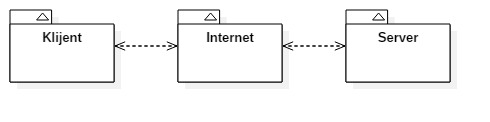
\includegraphics[scale=0.7]{images/dijagram1.jpg}
\end{center}
%% slika

\subsection{Korisnički interfejsi}

Korisnički interfejs omogućava kvalitetnu i jednostavnu komunikaciju korisnika sa aplikacijom. Kroz dizajn korisničkih interfejsa nastoji se osigurati da klijent na lak i intuitivan način dolazi do svih funkcionalnosti aplikacije. S obzirom da aplikacija ima samo jednu klasu korisnika, nužno je i omogućiti da korisnici bez problema dolaze do funkcionalnih zahtjeva koji se mogu grupisati u sljedeće kategorije:

\begin{enumerate}
    \item Upload .pdf dokumenata
    \item Pregled svih ranije dodanih dokumenata
    \item Otvaranje dokumenta i biranje ponuđenih opcija
\end{enumerate}

Više detalja oko korisničkih interfejsa će biti ponuđeno u jednom od narednih dijelova ovog dokumenta.


\section{Funkcionalnosti proizvoda}
\subsection{Upravljanje korisnicima}
Privilegije za kreiranje korisničkog računa ima svaka osoba koja ima pristup aplikaciji. Privilegiju za modifikovanje i brisanje postojećeg korisničkog računa ima samo korisnik. Upravljanje korisničkim računima uključuje:
\begin{itemize}
  \item Kreiranje novog korisničkog računa
  \item Modifikacija postojećeg korisničkog računa
  \item Brisanje postojećeg korisničkog računa
\end{itemize}

\subsection{Upload pdf fajlova}
Privilegiju za upload pdf fajlova imaju ulogovani korisnici. Upload pdf fajlova predstavlja preduslov za glavnu funkcionalnost sistema - čitanje. Funkcionalnosti koje su podržane, a vezane su za upload pdf fajlova su:
\begin{itemize}
  \item Importovanje online pdf dokumenta
  \item Importovanje pdf dokumenta sa lokalnog uređaja
  \item Prikaz svih korisnikovih pdf fajlova
  \item Pretraga i filtriranje dokumenata
\end{itemize}

\begin{center}
    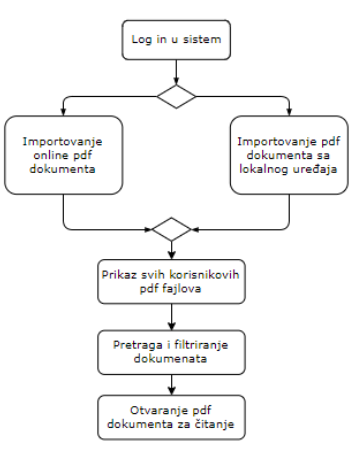
\includegraphics[scale=0.8]{images/FunkcionalniZahtjevi.png}
\end{center}


\subsection{Čitanje pdf fajlova}
Funkcionalnost čitanja pdf fajlova predstavlja centralnu funkcionalnost sistema i ona uključuje slijedeće:
\begin{itemize}
  \item Otvaranje pdf dokumenta za čitanje
  \item Čitanje pdf dokumenta
  \item Praćenje napretka čitanja pdf fajla
\end{itemize}

\subsection{Izdvajanje citata}
Privilegiju za izdvajanje citata iz određenog dokumenta imaju korisnici koji su ulogovani na svoj korisnički račun, u slučaju da legalno posjeduju pdf fajl. U sklopu ove  funkcionalnosti su:
\begin{itemize}
  \item Izdvajanje citata iz otvorenog pdf dokumenta
  \item Označavanje dijelova teksta promjenom boje ili pozadine teksta
  \item Arhiviranje citata u posebnom fajlu
  \item Komentarisanje dijelova pdf dokumenta
\end{itemize}


\subsection{Povezivanje sa mobilnom aplikacijom}
S obzirom na postojanje odgovarajuće mobilne aplikacije, sistem ima funkcionalnost redirekcije na istu. Odnosno:
\begin{itemize}
  \item Redirekcija na instalaciju mobilne verzije aplikacije
\end{itemize}




\section{Karakteristike korisnika}
Sistem, zbog svoje namjene i specifikacija, razlikuje samo jednu vrstu korisnika. U nastavku su opisane opšte karakteristike korisnika aplikacije, te potrebna znanja i iskustva za upravljanje, odnosno korištenje aplikacije.


\subsection{Korisnik aplikacije}
Korištenje sistema ne zahtjeva napredno znanje rada na računaru ili specijalnu obuku, jer je prilagođen za upotrebu svim profilima korisnika zainteresovanim za rad na ovoakvom tipu aplikacije. Dizajniran je da bude u skladu sa glavnim UI/UX principima, što ga čini intuitivnim i jednostavnim za korištenje širokom spektru tipova korisnika bez obzira na dob ili stepen tehnološke pismenosti.  \\ U cilju korištenja “Reader” softverskog rješenja, korisnik pravi svoj korisnički račun pomoću kojeg se prijavljuje na sistem i koristi njegove usluge. Te usluge, za korisnika, podrazumijevaju importovanje i pregled pdf dokumenata, čitanje dokumenata i podvlačenje njegovog sadržaja. S obzirom da se radi o web aplikaciji ona je dostupna u bilo kojem operaacionom okruženju koje ima internet konekciju. Korisnici ovo softversko rješenje mogu koristiti iz udobnosti svoga doma, na poslu, restoranu, ili gdje god im se ukaže potreba.\\ \\ Ovoj grupi korisnika dozvojeno je korištenje sljedećih funkcionalnosti:
\begin{enumerate}
    \item Registracija i login korisnika
    \item Importovanje pdf dokumenata sa lokalnog uređaja
    \item Importovanje online pdf dokumenata
    \item Pregled svih korisnikovih pdf dokumenata
    \item Čitanje pdf dokumenata i podvlačenje njegovog sadržaja
    \item Izdvajanje citata iz određenog dokumenta i arhiviranje istih u zasebnom odjeljku
    \item Ostavljanje komentara na dijelove pdf dokumenta
\end{enumerate}

U nastavku je prikazan use-case dijagram za korisnike aplikacije. \\

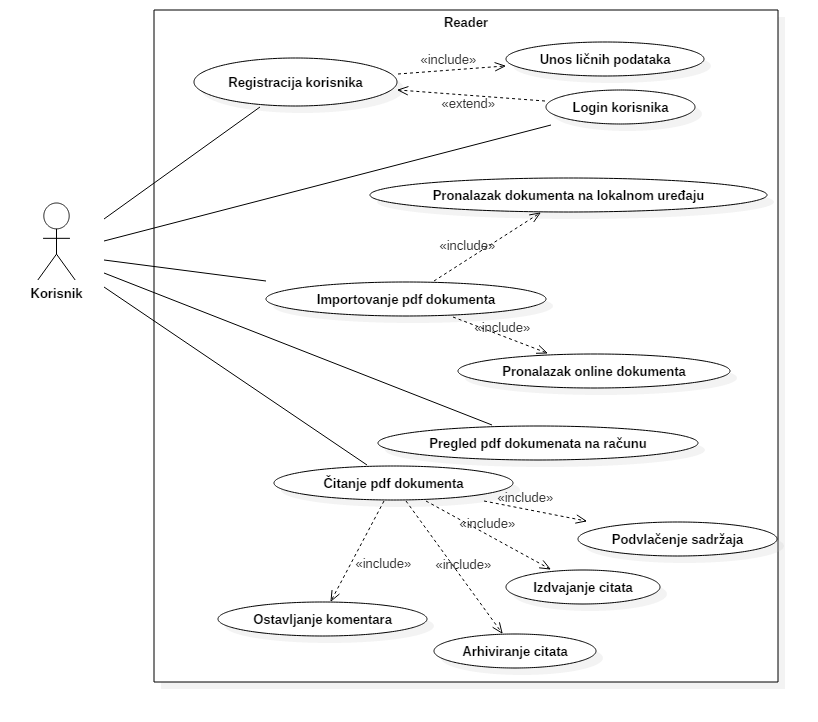
\includegraphics[scale=0.45]{images/UseCaseKorisnik.png}

\section{Ograničenja}

\subsection{Regulativni propisi}
Ovaj sistem će biti razvijen unutar zakonskih ograničenja koja postavlja Internacionalna Copyright Konvencija (ICC) iz 1952. Godine te Zakon o autorskim i srodnim pravima objavljenim u Službenom glasniku BiH broj 63/10. U skladu sa istim, aplikacija ne smije dozvoljavati modifikovanje sadržaja PDF fajlova.

\subsection{Hardverska ograničenja}
Za ispravno funkcionisanje aplikacije potrebno je da klijent ima adekvatnu mrežnu opremu i uspostavljenu vezu sa internetom te web browser koji je kompatibilan sa React.js frameworkom.

\subsection{Softverska ograničenja}
Za razvoj sistema potrebno je obezbijediti sljedeće:
\begin{itemize}

\item Klijentska aplikacija napisana u React.js frameworku sa kojom se vrši interakcija pomoću web browsera.

\item Internet konekcija je jedan od ključnih ograničenja za aplikaciju. Pošto aplikacija kupi podatke iz baze podataka preko interneta, potrebna je internet konekcija da bi aplikacija ispravno radila.

\item Web aplikacija će biti ograničena kapacitetom baze podataka i kapaciteta prostora alociranog za čuvanje PDF fajlova.

\item Ubuntu server 16.04.4 na kom će biti pokrenut DBMS (DataBase Management System)

\item Postgrade SQL 10.3 za upravljanje centralnom bazom podataka.

\item Serverska aplikacija će biti napisana u Node.js i Express framework-u te će usluživati klijentsku aplikaciju i moblinu aplikaciju.

\item Prilikom pravljenja aplikacije potrebno je voditi računa o privatnosti korisnika. Pošto je u pitanju web aplikacija, svi korisnički podaci će se čuvati na cloud serveru te je zbog toga potrebno preduzeti odgovarajuće mjere predostrožnosti da se isti zaštite.

\item Pošto će svi podaci i informacije biti čuvani na serveru kom će korisnici imati pristup, potrebno je limitirati korisničke privilegije i na taj način spriječiti mogućnost nanošenja štete drugim korisnicima i serveru.
\end{itemize}


\section{Pretpostavke i zavisnosti}
Da bi sistem uspješno funkcionisao potrebno je da su ispunjene naredne pretpostavke:
\begin{itemize}
    \item \textbf{Pretpostavka 1.} Pretpostavlja se da prije nije postojao sistem, tako da nije potrebno vršiti integraciju sa starim sistemom. 
    \item \textbf{Pretpostavka 2.} Pretpostavlja se da serverski računar ima obezbijeđeno stabilno napajanje 24 sata dnevno, prema preporukama iz zvanične dokumentacije serverskog hardvera, te da postoji UPS uređaj, koji će služiti kao rezervna mogućnost napajanja u slučaju nepredviđenih situacija.
    \item \textbf{Pretpostavka 3.} Pretpostavlja se da korisnički računar ima instaliran web browser i pristup internetu.
    \item \textbf{Pretpostavka 4.} Pretpostavlja se da korisnici ove aplikacije posjeduju osnovno poznavanje rada na računaru odnosno da posjeduju barem mjesec dana iskustva svakodnevnog korištenja nekog interfejsa, koji spada u grupu čovjek-računar interfejsa (eng. Human-Computer interface).
    \item \textbf{Pretpostavka 5.} Pretpostavlja se da  korisnik ima e-mail adresu pomoću koje kreira i verifikuje račun.
    \item \textbf{Pretpostavka 6.} Pretpostavlja se da će se korisnici sistema savjesno i odgovorno odnositi prema korisničkim podacima za prijavu na sistem, odnosno da niko drugi osim njih neće znati te podatke, te da podaci neće biti zloupotrijebljeni.
    \item \textbf{Pretpostavka 7.} Pretpostavlja se da ukoliko u toku ili nakon izrade sistema dođe do promjene zahtjeva ili dodatnih zahtjeva za funkcionalnostima, potrebno je pratiti korake koji su navedeni u poglavlju 2.6. Planiranje zahtjeva ovog dokumenta.
\end{itemize}

\section{Planiranje zahtjeva}
Zahtjevi koji su definisani u ovom dokumentu rezultat su analize korisničkih zahtjeva, razgovora sa korisnikom, te analiziranjem zakonskih regulativa. \\
U slučaju da naručilac sistema želi dodati, promijeniti ili izbaciti pojedine funkcionalnosti nakon zaključivanja specifikacije zahtjeva sistema, prati se naredna procedura:
\begin{itemize}
\item Naručioc sistema dužan je dostaviti zvanični zahtjev za promjenom funkcionalnosti, kojeg potpisuje ovlaštena osoba, a u kojem su detaljno definisane željene promjene.
\item DevTech se obavezuje da će najkasnije u roku od 10 dana nakon prijema zahtjeva, uraditi analizu traženih promjena i dostaviti odgovor naručiocu, odnosno ponudu za traženu promjenu, u kojoj će biti definisano koliko će promjena utjecati na cijenu izvedbe sistema i vremenski period predviđen za razvoj.
\item Ukoliko se naručioc složi sa dostavljenom ponudom, revidirana verzija SRS-a postaje obavezujuća za obje strane.
\item U slučaju da naručilac zahtjeva promjene nakon zaključivanja specifikacije zahtjeva sistema, DevTech zadržava pravo da ne pristane na izvršavanje traženih promjena.
\end{itemize}
U slučaju da razvojni tim želi dodati, promijeniti ili izbaciti pojedine funkcionalnosti sistema nakon zaključivanja specifikacije sistema, tada se prati naredna procedura:
\begin{itemize}
\item DevTech je dužan dostaviti zvanični zahtjev za promjenom funkcionalnosti naručiocu sistema, kojeg potpisuje ovlaštena osoba, a u kojem su detaljno definisane željene promjene i njihov uticaj na cijenu sistema i planirani vremenski period za razvoj softvera.
\item Naručioc sistema dužan je najkasnije u roku od 15 dana od dana prijema zahtjeva, izjasniti se o promjeni.
\item Ukoliko se naručioc složi sa upućenim zahtjevom, revidirana verzija SRS-a postaje obavezujuća za obje strane.
\end{itemize}